<<<<<<< HEAD
\documentclass[conf]{new-aiaa}
%\documentclass[journal]{new-aiaa} %for journal papers
=======
%\documentclass[conf]{new-aiaa}
\documentclass[journal]{new-aiaa} %for journal papers
>>>>>>> 43cfb1abf9193b239f9fc20d6944e361c25605f8
\usepackage[utf8]{inputenc}

\usepackage{graphicx}
\usepackage{amsmath}
\usepackage[version=4]{mhchem}
\usepackage{siunitx}
\usepackage{longtable,tabularx}
\setlength\LTleft{0pt} 
\usepackage{subcaption}
\usepackage{float}




%\usepackage[utf8]{inputenc}
%\usepackage[english]{babel}
%
%\setlength{\parindent}{4em}
%\setlength{\parskip}{1em}
%\renewcommand{\baselinestretch}{1.5}



\title{Fly-Back of a Scramjet-Powered Accelerator}

 \author{
 	Sholto O. Forbes-Spyratos%
 	\footnote{Ph.D. Candidate, Centre for Hypersonics, School of Mechanical and Mining Engineering. Member AIAA.}
 	\ ,  Michael P. Kearney
 	\footnote{Lecturer, School of Mechanical and Mining Engineering.}
 	\ ,  Michael K. Smart
 	\footnote{Professor, Centre for Hypersonics, School of Mechanical and Mining Engineering. Senior Member AIAA.}
 	\ and   Ingo H. Jahn
 	\footnote{Lecturer, Centre for Hypersonics, School of Mechanical and Mining Engineering. Member AIAA.}
 	\\
 	{\normalsize\itshape
 		The University of Queensland, Queensland, Australia, 4072}\\
 }

\begin{document}

\maketitle

\begin{abstract}

\end{abstract}

\section{Nomenclature}

{\renewcommand\arraystretch{1.0}
\noindent
\begin{longtable*}{@{}l @{\quad=\quad} l@{}}
 $t$ & Time (s)\\
 $q$ & Dynamic Pressure (Pa)\\
 $F$ & Force (N)\\
 $\rho$& Density (kg/m$^2$)\\
 $C_L,C_D$ & Aerodynamic Coefficients\\
  $v$ & Velocity (m/s)\\
  $A$ & Reference Area (m$^2$)\\
 $r$ & Radius from Earth Centre (m)\\
 
 $\gamma$& Trajectory Angle (rad)\\
 $\omega$ & Angular Velocity (rad/s)\\
 $m$  & Mass (kg)\\
 $T$ & Thrust (N)\\
 
 $\xi$ & longitude (rad)\\
 $\phi$ & latitude (rad)\\
  $\gamma$ & flight path angle (rad)\\
  $v$ & velocity (m/s) \\
   $\zeta$ & heading angle (rad)\\
   $\mu_E$ & Standard Gravitational Parameter ($m^3/s^2$)\\
\end{longtable*}}

\newpage
\section{Introduction}

The decreasing size and cost of satellites is driving an upsurge in the number of small satellite launches\cite{Faa&Ast&Comstac2015}\cite{Maddock2016}. Many of these small satellites require custom orbits, which are specified by the satellite manufacturer. These custom orbits often require specific orbital inclinations, and have small launch windows. Satellites which form part of constellations are particularly sensitive to launch conditions due to the requirement for them to fit into a complex orbital schedule\cite{Crisp2015}. Launchers which can deliver a small payload into a custom orbit, at short notice, are in increasing demand, and are being investigated or developed by a number of organisations\cite{Linkspace,DARPA2017,Lynx,Maddock2017,Kuhn2017,charania,Gilmour,Bloostar,Virgin,Firefly, Electron}. These small satellite launchers offer the user flexibility in orbit and launch schedule, at comparable cost-per-kg to piggybacking on larger launches. 

Currently all small launchers are expendable, however, the development of reusable or partially reusable launch systems has recently flourished, led by SpaceX, and fuelled by the need to decrease launch costs and turnaround times. Incorporating reusability into the design of small satellite launchers is complicated, due to the scaling difficulties posed by reusable systems. The feasibility of reusable small launchers is being investigated, with  both vertical landing \cite{Linkspace} and horizontal landing \cite{DARPA2017,Lynx} rocket-powered concepts under development. 

 The University of Queensland and Hypersonix are developing a rocket-scramjet-rocket multi stage launch system for small satellite launches, incorporating the SPARTAN\cite{Preller2017} as the second stage. 
\begin{figure}
	\centering
	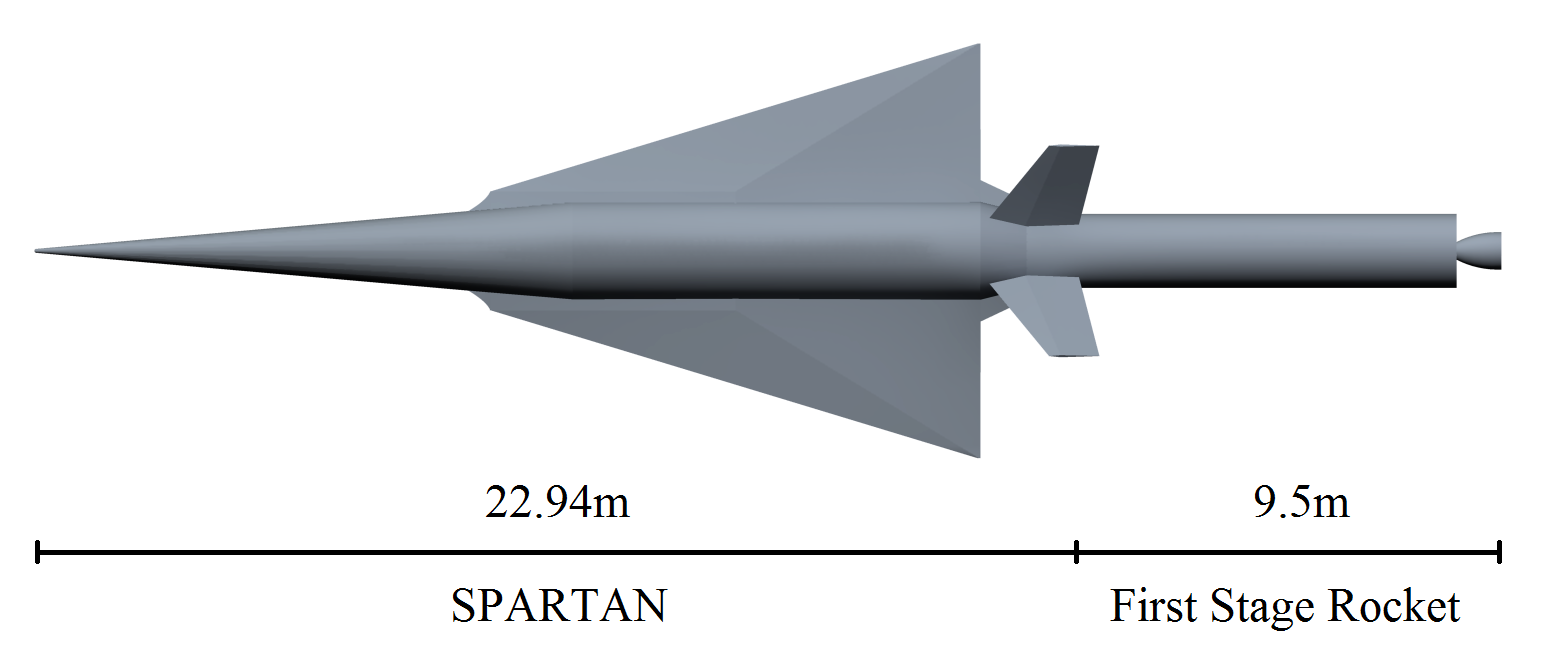
\includegraphics[width=0.7\linewidth]{Figures/NoInternal}
	\caption{The rocket-scramjet-rocket access-to-space system, including the SPARTAN accelerator \cite{ForbesSpyratos2018}.}
	\label{fig:NoInternal}
\end{figure}
\begin{figure}
	\centering
	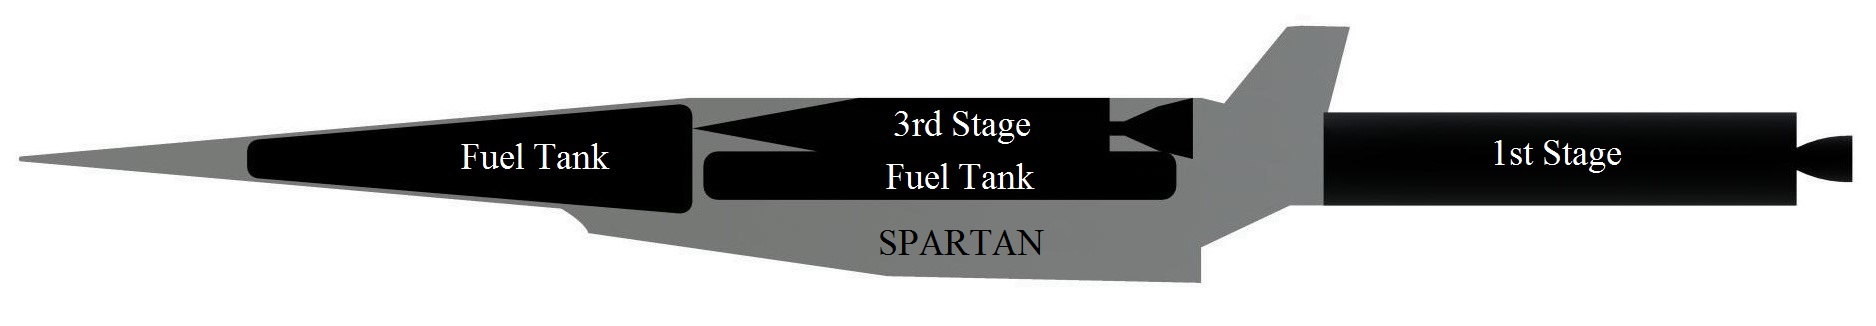
\includegraphics[width=0.7\linewidth]{Figures/INTERNALS}
	\caption{Side view of the rocket-scramjet-rocket system including internals of the SPARTAN vehicle \cite{ForbesSpyratos2018}.}
	\label{fig:INTERNALS}
\end{figure}
The SPARTAN is a scramjet-powered accelerator designed to operate between approximately Mach 5 and Mach 9. It is accelerated to Mach 5 by a rocket-powered first stage, and at the end of the acceleration phase, a rocket-powered third stage is separated which carries a payload to orbit.
The SPARTAN has a total length of 22.94m, a wingspan of 8.9m and weighs a total of 9819kg, including the third stage.  
Four underslung C-REST scramjet engines are used to power the SPARTAN, sized to a capture width of 0.65m \cite{Preller2017}.
The SPARTAN carries 1562kg of LH2 propellant in three tanks, shown in Figure \ref{fig:INTERNALS}, one designed to fit in the nose cone, and two to fit within the fuselage underneath the third stage vehicle. 

The use of a scramjet engine improves the specific impulse of the SPARTAN compared to rocket-powered vehicles, and eliminates the necessity for oxidiser to be carried on board. Carrying only fuel on board the vehicle allows the SPARTAN to have a design similar to a traditional aircraft, including avionics and landing gear. The aerodynamic capabilities and avionic systems of the scramjet stage allow it to return to its initial launch site, and land horizontally on a traditional runway. After landing, the vehicle is checked and re-fuelled, and is then ready to launch again. The increased reusability that this affords over similarly sized launch systems reduces the cost-per-kg of launch. 

\begin{figure}
\centering
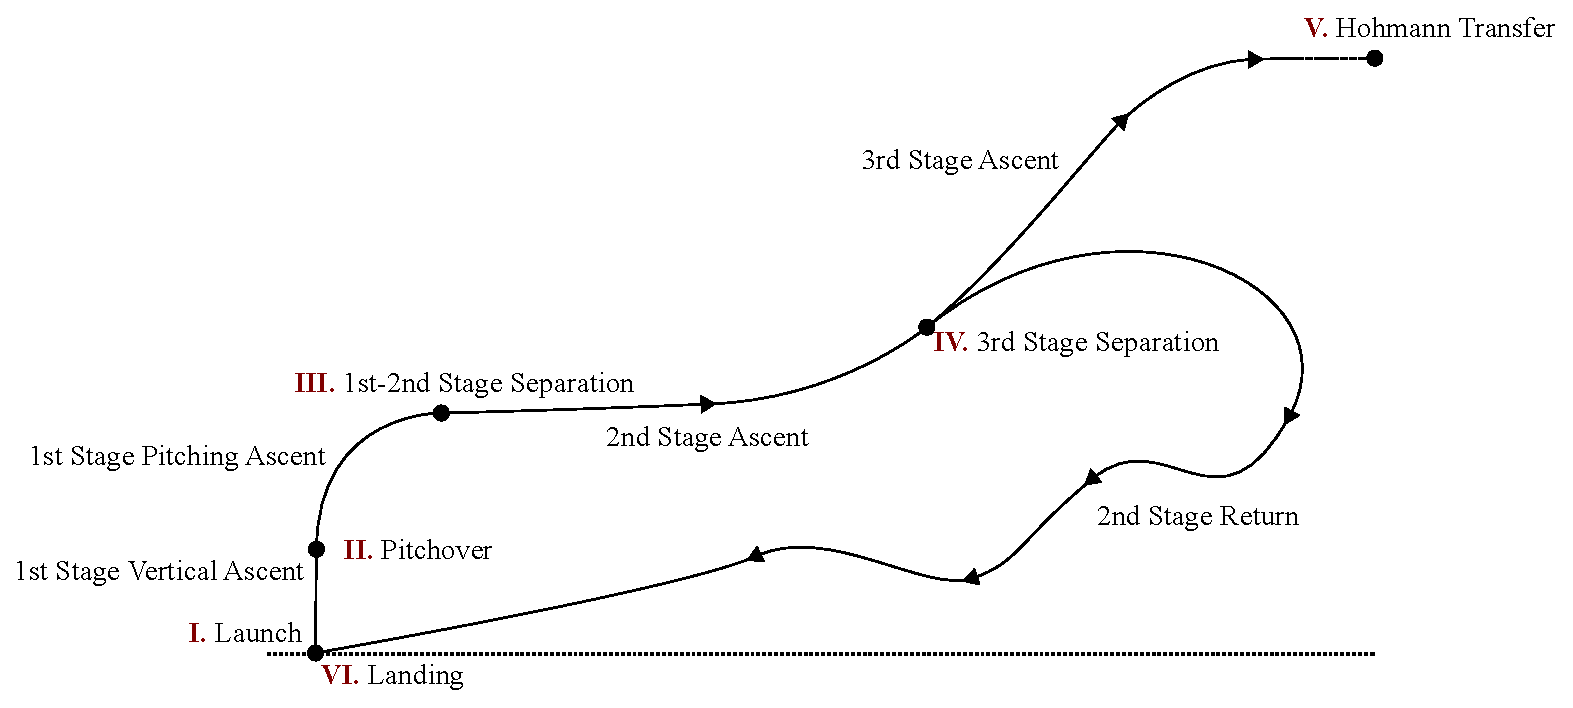
\includegraphics[width=0.9\linewidth]{Figures/Traj}
\caption{A representative view of the trajectory of the rocket-scramjet-rocket launch system incorporating the SPARTAN accelerator.}
\label{fig:Traj}
\end{figure}


The trajectory of the rocket-scramjet-rocket launch system is shown in Figure \ref{fig:Traj}. The system launches vertically under rocket power, and pitches over until close to horizontal flight. The SPARTAN separates from the first stage rocket at Mach 5.1, the minimum operable Mach number of the scramjet engines. It then accelerates until approximately Mach 9, at which time a pull-up manoeuvre is performed and the third stage rocket is released. The third stage rocket then accelerates, exits the atmosphere, and performs a circularisation burn. At this point a Hohmann transfer is performed to reach the desired orbit. Meanwhile, the SPARTAN turns and flies back to the initial launch site.
The ascent profile of the rocket-scramjet-rocket system incorporating the SPARTAN vehicle has been analysed and optimised in previous studies \cite{Preller2017,ForbesSpyratos2018}. However, these studies do not incorporate the return flight of the SPARTAN. The fly-back is crucial to the feasibility of the system, as the cost efficiency of the SPARTAN depends on its reusability and short turnaround time.
The fly-back of the SPARTAN must be analysed to ensure that the full reusability of the SPARTAN is achievable. 



To maximise fuel efficiency, it is desirable for the SPARTAN to perform a minimum-fuel fly-back to the initial launch site, with the best-case scenario being for the fly-back to use no fuel at all.
 However, for a hypersonic trajectory a fully glide-back return flight is most likely unobtainable. This is due to the large downrange distance flown, and the large initial velocity at the beginning of the fly-back trajectory, when the vehicle is oriented away from the landing site.
In previous studies, the maximum separation velocity for glide-back to be feasible has been found to be between Mach 3-4 at 30km-120km downrange distance, with higher initial velocities or longer downrange distances requiring fly-back under power\cite{Hellman,Tetlow1992}.
Powered fly-back may be achieved either through the use of the existing airbreathing engines, or by using additional engines added for the fly-back only\cite{Mehta2001,Tetlow1992,Hellman,Wilhite1991}. 
The addition of subsonic engines powering a constant velocity cruise-back phase allows the accelerator to return to base with a similar trajectory to that of traditional aircraft, allowing the velocity and altitude of the accelerator to be precisely controlled. However, the addition of subsonic engines necessary for cruise-back increases the mass of the vehicle significantly, leading to decreased mass efficiency and increased design complexity\cite{Hellman}. 
A preferable mode of powered fly-back is to use the existing hypersonic airbreathing engines during the return trajectory. Using the existing airbreathing engines allows for range to be added to the return trajectory, without the inclusion of additional engines. The hypersonic airbreathing engines can be operated at appropriate times during the fly-back, when they will be most impactful on the return trajectory range. However, the hypersonic airbreathing engines may only be used within their operating region, and vary in thrust and efficiency dependent on flight conditions. Hypersonic airbreathing engines have maximum efficiency at low Mach numbers\cite{Preller2017}, with the thrust produced depending on the dynamic pressure and inlet conditions, which vary with the trajectory path and angle of attack of the vehicle. This added complexity requires the use of trajectory optimisation methods to find the most efficient flight path for return to the launch site, and to ensure that the return of the vehicle under its own power is viable. 


Vehicles using high-speed airbreathing propulsion in return flight are investigated in a study by Tsuchiya and Mori\cite{Tsuchiya2005}.  Tsuchiya and Mori investigate two conceptual launch vehicles; a vehicle powered solely by airbreathing propulsion returning after separation of an orbital stage at Mach 5.1, and an airbreathing/rocket vehicle returning after a separation at Mach 6.8\cite{Tsuchiya2005}. 
These boosters fly to a downrange distance of 600-625km from the launch site, and separate from the orbital accelerator at a dynamic pressure of 15kPa\cite{Tsuchiya2005}. At the start of their respective return trajectories, both boosters turn with a bank angle of 130-145$^\circ$. Both the fully-airbreathing and partially-airbreathing vehicles ignite their airbreathing engines for 'several tens of seconds' at approximately Mach 3.5, in order to extend the flight range of the vehicles and return to the initial launch site\cite{Tsuchiya2005}. Less than 5\% of the vehicles initial propellant was required to return the vehicles to the initial launch sites\cite{Tsuchiya2005}.

When compared to the vehicles investigated by Tsuchiya and Mori\cite{Tsuchiya2005}, the SPARTAN separates from its third stage rocket at a considerably higher Mach number of Mach 9.1, as well as at a considerably higher dynamic pressure of 33.9kPa. The SPARTAN must also cover a longer fly-back range of 878km. In addition, the C-REST scramjet engines are limited to operating at hypersonic speeds of Mach 5.1 or higher. These design differences create substantially more challenging conditions than those studied by Tsuchiya and Mori. Consequently, it is necessary to investigate the ability of the SPARTAN to return to the launch site following separation. 

The aim of this paper is to find the minimum-fuel fly-back trajectory for the SPARTAN vehicle using trajectory optimisation. The feasibility of the fly-back trajectory is assessed from a representative third stage separation location, and the sensitivity of the fly-back trajectory to variation of vehicle parameters is investigated. 







%\subsection{Third Stage}

%The third stage rocket weighs a total of 3300kg, and is powered by a SpaceX LOX-kerosene Kestrel engine, weighing 52kg. The third stage rocket is protected while in-atmosphere by a heat shield weighing 130.9kg. The heat shield is constructed from a phenolic cork cylinder, carbon-carbon nose cone, and tungsten tip. When the third stage reached 10pa the heat shield is discarded, as aerodynamic heating is assumed to be negligible at this point. 
%\begin{figure}
	%\centering
	%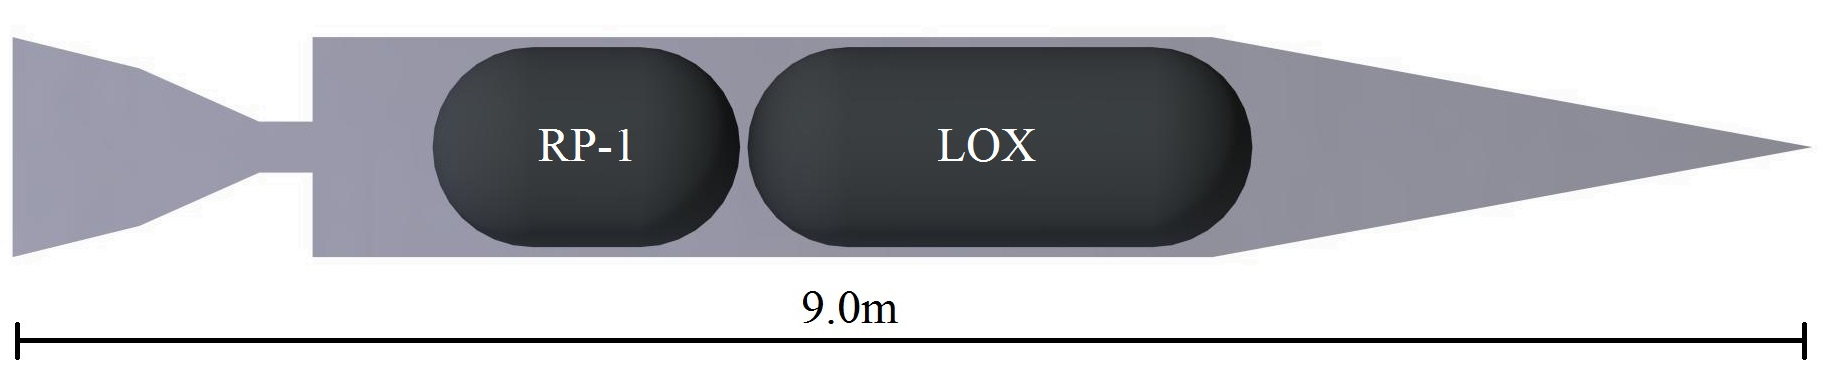
\includegraphics[width=0.7\linewidth]{Figures/3rdStage}
	%\caption{}
	%\label{fig:3rdStage}
%\end{figure}



\section{Aerodynamics}\label{sec:aero}

 \begin{figure}
 	\centering
 	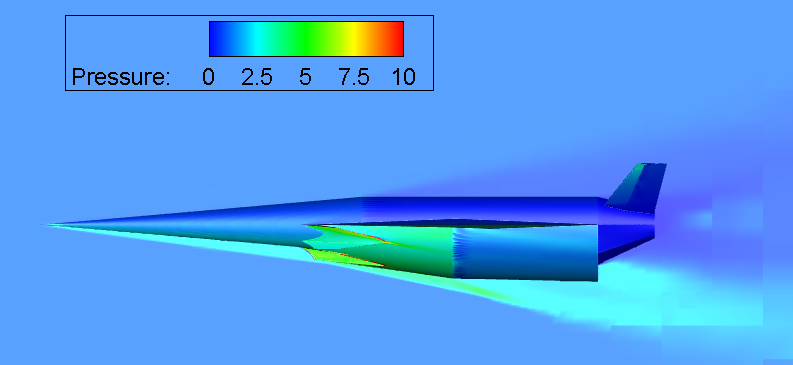
\includegraphics[width=0.7\linewidth]{Figures/M7AoA6}
 	\caption{Normalised pressure contours around the SPARTAN accelerator calculated using CART3D, for Mach 7, 6$^\circ$ angle of attack flight}
 	\label{fig:M7AoA6}
 \end{figure}

 This study utilises CART3D to calculate the aerodynamics of the SPARTAN vehicle\cite{CART3D}. CART3D is an inviscid CFD solver for the preliminary design of aerospace vehicles. CART3D utilises adjoint-based mesh refinement with a Cartesian cut-cells approach to produce an iteratively refined mesh to fit a flow solution\cite{Aftosmis1997}. CART3D has been used to generate the aerodynamic database of the SPARTAN vehicle due to its applicability in both the subsonic and supersonic regimes, and its robustness across multiple flow solutions \cite{ForbesSpyratos2018}. CART3D has previously been used to analyse hypersonic vehicles, and has shown good agreement with experimental data across multiple studies \cite{Sagerman2017,Aftosmis2011}. The SPARTAN has been simulated in CART3D across Mach numbers from 0.2 to 9, and for angle of attack values from 0$^\circ$ to 10$^\circ$. An example case is shown in Figure \ref{fig:M7AoA6}, for Mach 7, 6$^\circ$ angle of attack. Figures \ref{fig:Cl} and \ref{fig:Cd} show the lift and drag coefficients of the SPARTAN vehicle over the range of Mach numbers and angle of attack values analysed. 
 
 
 
 
 \begin{figure}
 	\centering
 	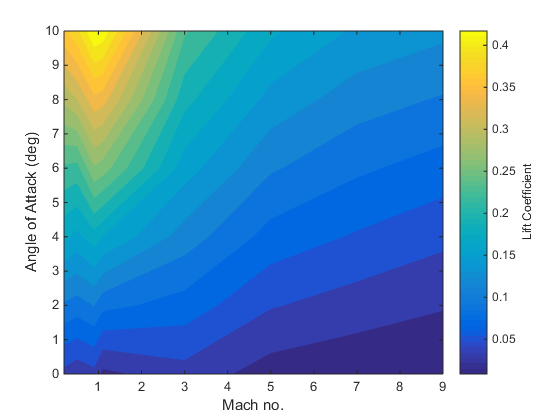
\includegraphics[width=0.6\linewidth]{Figures/Cl}
 	\vspace{-10pt}
 	\caption{Lift coefficient of the SPARTAN accelerator calculated using CART3D, over the flight range of Mach number and angle of attack values. $A_{ref} = 62.77m^2$.}
 	\label{fig:Cl}
 \end{figure}
 
 \begin{figure}
 	\centering
 	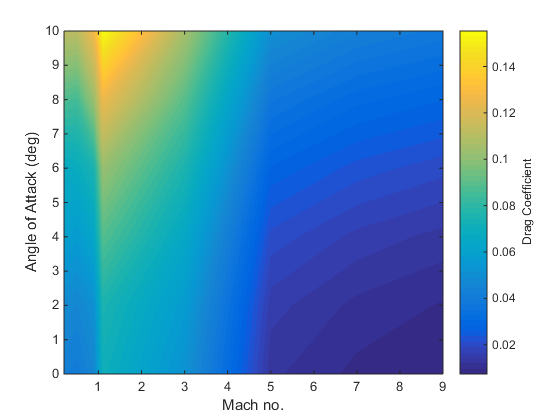
\includegraphics[width=0.6\linewidth]{Figures/Cd}
 	\vspace{-10pt}
 	\caption{Drag coefficient of the SPARTAN accelerator calculated using CART3D, over the flight range of Mach number and angle of attack values. $A_{ref} = 62.77m^2$.}
 	\label{fig:Cd}
 \end{figure}
 
 \begin{figure}
 	\centering
 	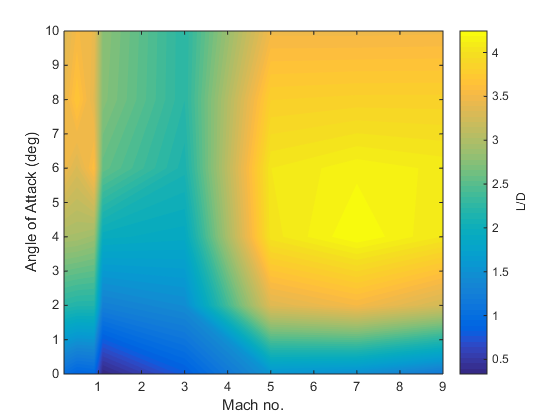
\includegraphics[width=0.6\linewidth]{Figures/LD}
 	\vspace{-10pt}
 	\caption{L/D of the SPARTAN accelerator calculated using CART3D, over the flight range of Mach number and angle of attack values. }
 	\label{fig:LD}
 \end{figure}
 
 
 
 For the purposes of this study, a point mass model is used in conjunction with the aerodynamic database, and atmospheric properties obtained from the U.S Standard Atmosphere 1976\cite{Administration1976}. The SPARTAN is assumed to be trimmed at all conditions during flight.
 

\section{Trajectory Optimisation}\label{sec:opt}
The optimisation of the trajectories in this study are performed using LODESTAR. LODESTAR is a trajectory optimisation tool under development at The University of Queensland for hypersonic vehicle analysis \cite{ForbesSpyratos2018}. LODESTAR generates optimal trajectories given a target cost function, and sets of initial and end constraints. LODESTAR utilises the pseudospectral method optimisation software GPOPS-2\cite{Patterson2015}. 

The pseudospectral method is a form of direct spectral collocation, in which a spectral collocation method is used to approximate the optimal control problem as a nonlinear programming problem. The pseudospectral method offers an accurate, robust optimal control solution with relatively good computational times\cite{Fahroo2000,Ross2004}, making it particularly applicable to complex hypersonic vehicle trajectories.  The pseudospectral method has been successfully applied in a variety of aerospace applications, and GPOPS-2 is used widely within the aerospace field as a solver for complex aerospace vehicle trajectories.


\subsection{Dynamic Model}

The SPARTAN is simulated in a geodetic rotational reference frame \cite{Josselyn2002a}: 

\begin{equation}
\dot{r} = v \, \sin \gamma
\end{equation}

\begin{equation}
\dot{\xi} = \frac{v \, \cos \gamma \, \cos \zeta}{r \, \cos \phi}
\end{equation}

\begin{equation}
\dot{\phi} = \frac{v\,\cos\gamma\,\sin\zeta}{r}
\end{equation}
\begin{equation}
\dot{\gamma} = \frac{T\,\sin\alpha}{m\,v}+ (\frac{v}{r}-\frac{\mu_E}{r^2 \,v})\,\cos\gamma + \frac{L}{m\,v}
+ \cos\phi[2\,\omega_E\, \cos\zeta + \frac{\omega_E^2\, r}{v}(\cos\phi\,\cos\gamma+\sin\phi\,\sin\gamma\,\sin\zeta)]
\end{equation}
\begin{equation}
\dot{v} = \frac{T\,\cos\alpha}{m}-\frac{\mu_E}{r^2}\,\sin\gamma - \frac{D}{m}
+ \omega_E^2 r\,\cos\phi(\cos\phi\,\sin\gamma-\sin\phi\,\cos\gamma\,\sin\zeta)
\end{equation}
\begin{equation}
\dot{\zeta} = -\frac{v}{r}\tan\phi\,\cos\gamma\,\cos\zeta +2\,\omega_E\,\cos\phi\,\tan\gamma\,\sin\zeta - \frac{\omega_E^2 r}{v\,\cos\gamma}\,\sin\phi \, \cos\phi\,\cos\zeta-2\omega_E\,\sin\phi 
\end{equation}

Where $r$ is the radius from the centre of Earth, $\xi$ is longitude, $\phi$ is latitude, $\gamma$ is flight path angle,$v$ is velocity and $\zeta$ is heading angle. The drag and lift of the SPARTAN are calculated using the standard aerodynamic coefficients;
\begin{equation}
F_d = \frac{1}{2} \, \rho \, C_D \, v^2 \, A ,
\end{equation}
\begin{equation}
F_L = \frac{1}{2} \, \rho \, C_L \, v^2 \, A ,
\end{equation}
where the coefficient of lift and drag are determined from the aerodynamic database described in Section \ref{sec:aero}.

\subsection{Third Stage Optimisation}

-details of third stage

-plot of payloads



\section{Trajectory Analysis}

-change this to be focussed on the combined trajectory


The trajectory of the SPARTAN is optimised using LODESTAR. 
The trajectory is optimised for maximum payload-to-orbit, with the fly-back end position constrained to be near to the initial launch site, close to  15.3$^\circ$S,144.9$^\circ$E\cite{ForbesSpyratos2018}. 

A small margin is allowed so as to not over-constrain the end position within LODESTAR, and it is assumed that the landing strip will not be at the exact location of the launch site. The angle of attack is limited to 10$^\circ$, to ensure vehicle stability. The bank angle is limited to 90$^\circ$ to produce a conservative solution and to limit any possible design complications that may arise from inverted flight. The dynamic pressure is limited to 50kPa, the structural limit of the vehicle. The scramjet engines are limited to only operate when the inlet dynamic pressure is above 20kPa, an estimated lower limit on the operable mass flow rate.
The end of the trajectory is constrained to sub-200m altitude, and a trajectory angle range between -10$^\circ$ and 0$^\circ$ to ensure that the SPARTAN can perform a landing manoeuvre. These constraints ensure that the vehicle is approaching the landing site at the end of the optimised trajectory. The end velocity is only limited to be greater than 0m/s. It can be assumed that the optimal fly-back trajectory minimises end velocity as shown in the optimised trajectory results. 
It is also assumed that the vehicle is able to carry any necessary fuel in addition to the fuel required during the ascent trajectory, allowing the initial conditions to be kept constant. The potential specific impulse is shown along the trajectory, this is the specific impulse obtainable from the C-REST engines should they be powered on.

\subsection{Optimised Trajectory}
-Put picture and discussion of full trajectory here

\subsection{Ascent}

\subsection{Fly-Back}
\begin{figure}[t]
	\centering
	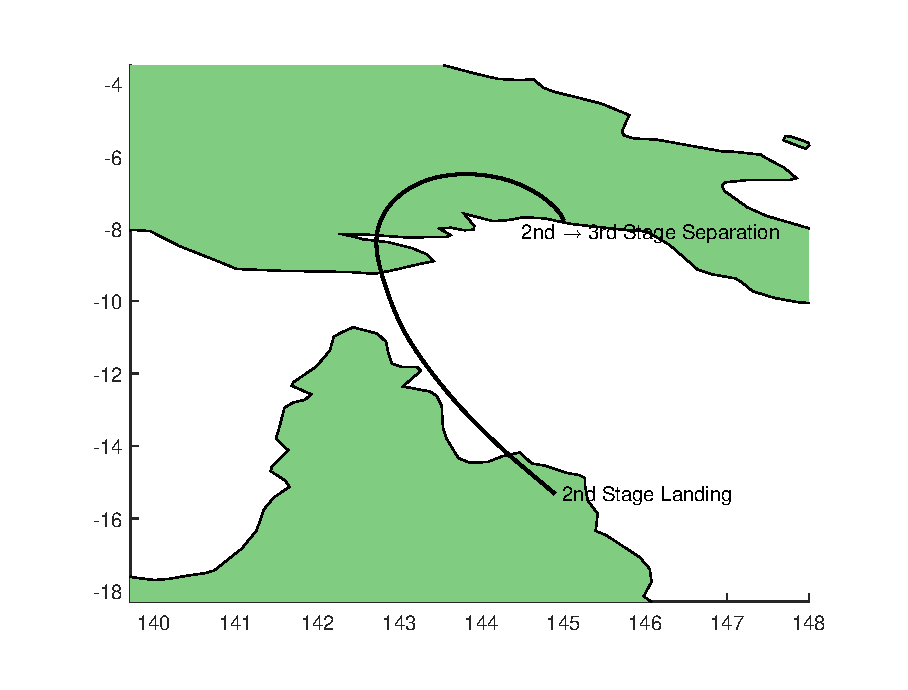
\includegraphics[width=0.6\linewidth]{Figures/lon-lat}
	\vspace{-10pt}
	\caption{ Ground track of the optimised fly-back of the SPARTAN vehicle.}
	\label{fig:lon-lat}
\end{figure}  


\begin{figure}
\begin{subfigure}[b]{\textwidth}
	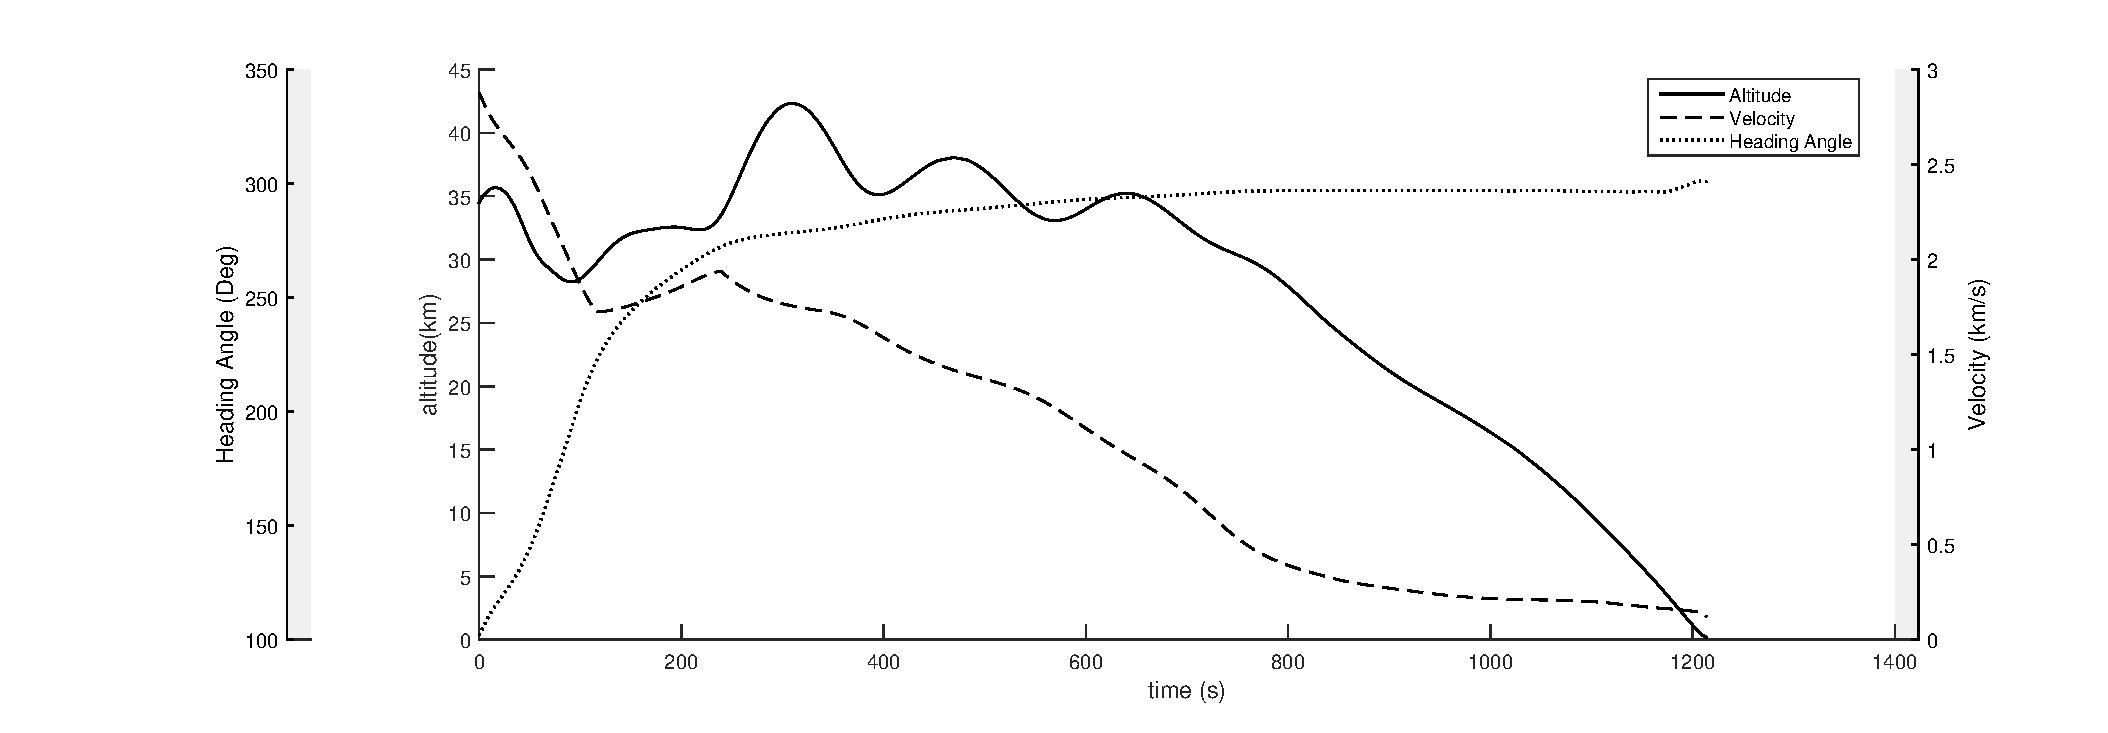
\includegraphics[width=\linewidth]{Figures/Traj1}
	\vspace{-15pt}
	\caption{ Flight path.}
	\label{fig:Traj1}
\end{subfigure}

\begin{subfigure}[b]{\textwidth}
	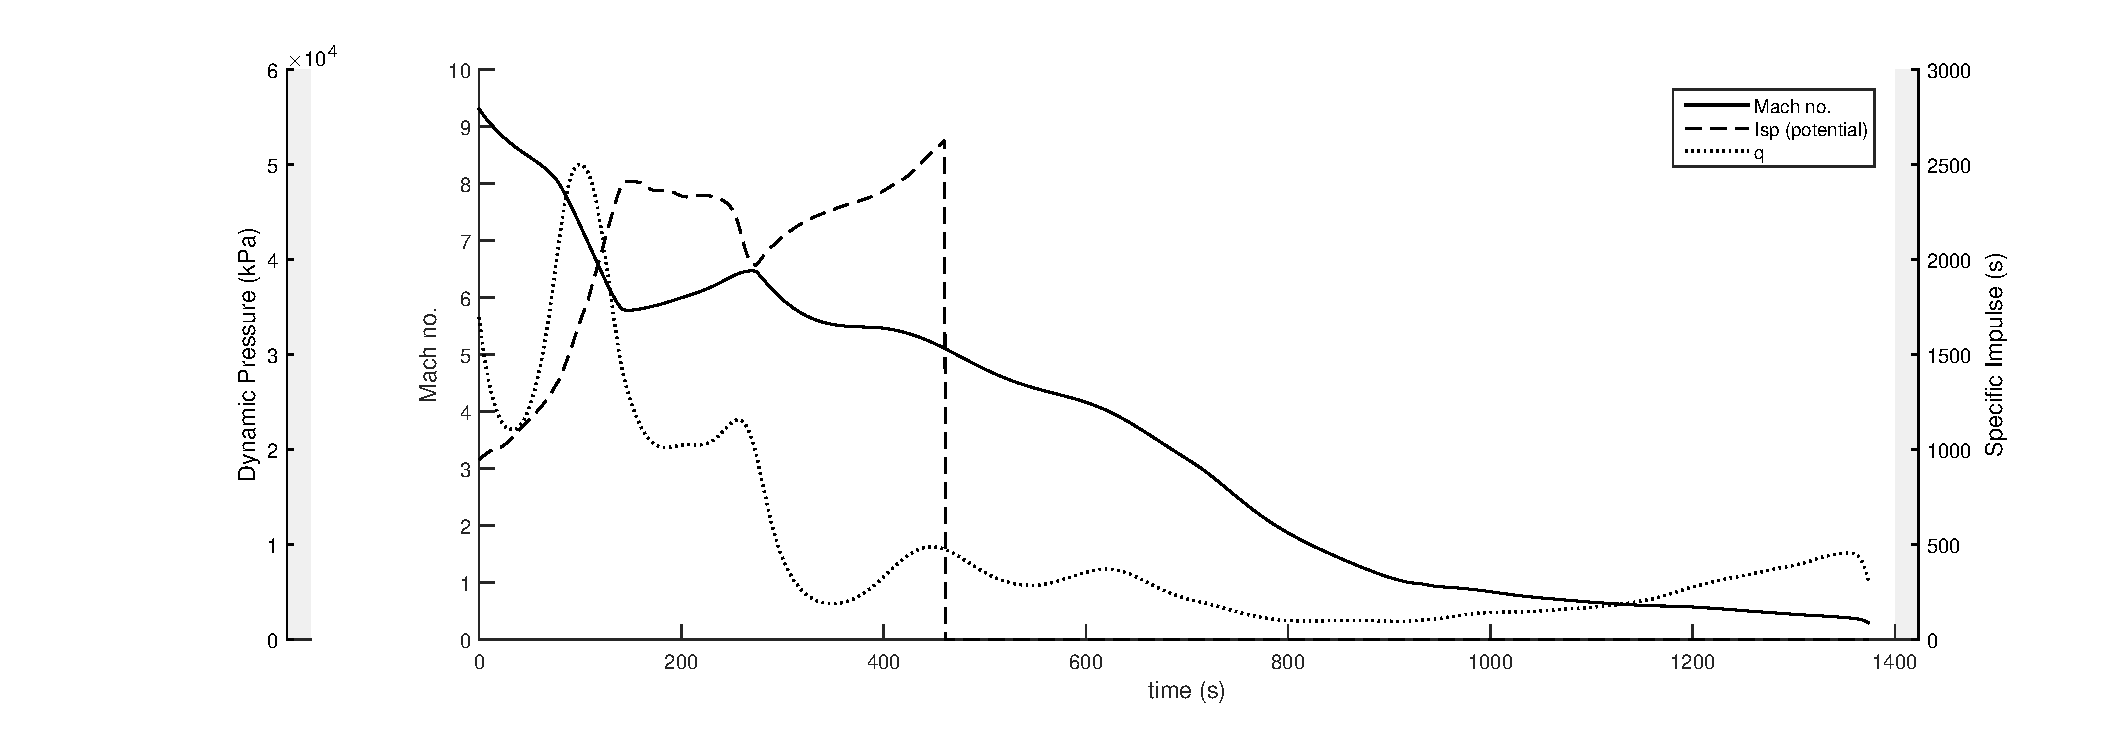
\includegraphics[width=\linewidth]{Figures/Traj2}
	\vspace{-15pt}
	\caption{Aerodynamic and performance data. }
	\label{fig:Traj2}
\end{subfigure}

\begin{subfigure}[b]{\textwidth}
	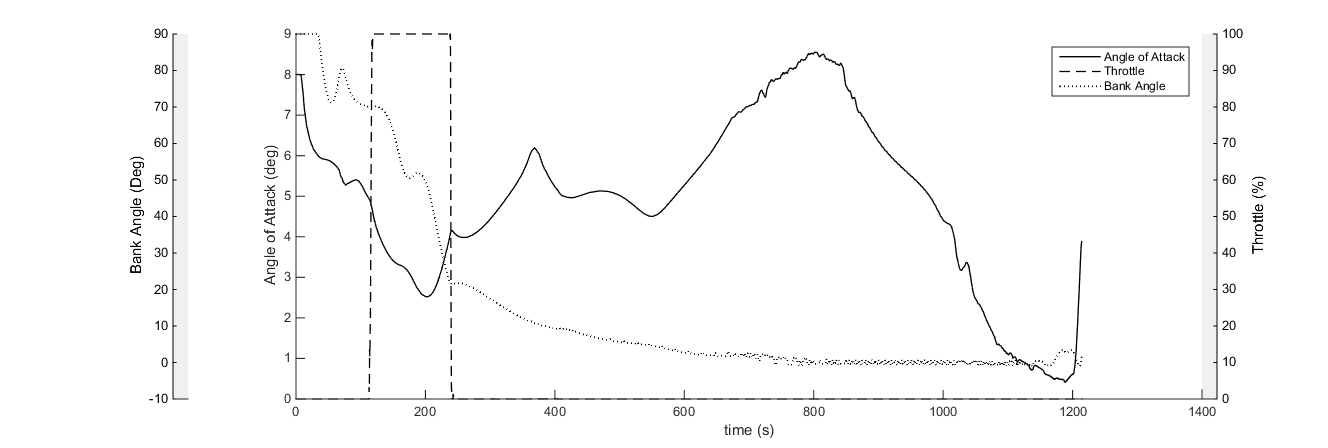
\includegraphics[width=\linewidth]{Figures/Traj3}
	\vspace{-15pt}
	\caption{Control time histories.}
	\label{fig:Traj3}
\end{subfigure}
\caption{Trajectory data for the fly-back of the SPARTAN vehicle. Optimised for minimum fuel usage using LODESTAR.}
\label{fig:AllTraj}
\end{figure}

The optimised fly-back trajectory is shown in Figures \ref{fig:lon-lat} and \ref{fig:AllTraj}.
The fly-back is initiated from the optimised second-third stage separation point at 7.7$^\circ$S,145.0$^\circ$E, 34.5km altitude, 2.9$^\circ$ trajectory angle, 2881m/s velocity and 102$^\circ$ heading angle, corresponding to the conditions of optimal third stage release described in Section \ref*{sec:opt}. 
The SPARTAN is shown to be capable of fly-back, using 166.0kg of fuel, a total increase in the fuel usage of the SPARTAN of 10.6\%.
The optimised trajectory has four distinct parts; 1. initial turn, 2. boost phase, 3. hop-glide, and 4. approach. 

\subsubsection{ Initial Turn}
The SPARTAN starts at the maximum bank angle of 90$^\circ$, and sustains this bank angle for 34.4s. At this point, the altitude of the SPARTAN decreases, and the vehicle is close to hitting the dynamic pressure of 50kPa. To avoid exceeding this limit, the bank angle is reduced to 71.2$^\circ$, allowing the vehicle to generate sufficient lift to slow its descent. The bank angle in then increased again, to 80.7$^\circ$ at 70.8s. After this time, the bank angle is gradually reduced. 

\subsubsection{ Boost Phase}
Soon after the bank angle begins to reduce, at 118.7s flight time and Mach 5.71, the scramjet engines are ignited. The C-REST engines are powered-on at a point of high potential specific impulse, at a low Mach number, and burn for 119.8s. The altitude of the SPARTAN is raised during the majority of the burn, ensuring that the Mach number is kept low for maximum efficiency\cite{Preller2017}, as shown in Figure \ref{fig:AllTraj}. The maximum altitude is limited by the lower dynamic pressure limit of the C-REST engines of 20kPa. The bank angle of the vehicle is reduced to produce increased lift, so as to increase the altitude of the SPARTAN, while also maximising the specific impulse of the scramjet engines by keeping the angle of attack low. Low angle of attack decreases the temperature and raises the Mach number, at the inlet of the C-REST engines. While these effects partially offset each other\cite{Preller2017}, the temperature increase is more significant, and decreasing angle of attack has the net effect of increasing the specific impulse of the C-REST engines. This increase in specific impulse is balanced by a decrease in the L/D of the SPARTAN at angle of attack values lower than 4$^\circ$, as illustrated in Figure \ref{fig:LD}. However, the specific impulse has a more significant impact than L/D during this phase, resulting in the optimised angle of attack being kept low. At 204s the angle of attack is increased, bringing the L/D of the vehicle towards maximum and initiating the first 'skip' of the skip-glide phase.  

<<<<<<< HEAD
NOTE Angle of attack is minimised to reduce q, not just for increased Isp
\subsubsection{3. Skip-Glide}
=======

\subsubsection{ Skip-Glide}
>>>>>>> 43cfb1abf9193b239f9fc20d6944e361c25605f8
During the unpowered trajectory after the burn phase, the angle of attack is controlled so that the L/D of the SPARTAN is close to the maximum. Initially, the SPARTAN performs several 'skips' after the scramjet burn. These are due to the high L/D of the SPARTAN above Mach 4, and are aided by the angle of attack, which is controlled to emphasize the size of the skips. These skips are consistent with research which has shown that a periodic skipping trajectory increases the downrange distance achievable by hypersonic vehicles\cite{Eggers1957,Kanda2007}. 


\subsubsection{ Approach}
After the skip phase, as the vehicle is approaching Mach 1, the angle of attack is reduced gradually to bring the SPARTAN down to 200m altitude, in a controlled manner. 
 At the end of the trajectory the SPARTAN levels out, and reaches 200m altitude at -9.6$^\circ$ trajectory angle and 119.8m/s velocity. These conditions are similar to those of the space shuttle at landing\cite{Ryba2017}, and it is assumed that the SPARTAN is able to perform a landing manoeuvre after this point. 





\section{Sensitivity Analysis}
-\textbf{REDO THIS TO BE FROM COMBINED OPTIMISED SEPARATION POINT}
-Check that fuel-mass optimised flyback is reasonably consistent with combined payload-optimised optimised result
-Should I even look at 

To investigate the robustness of the fly-back trajectory to vehicle design; the drag coefficient and specific impulse of the SPARTAN are varied by $\pm 10\%$, and the new optimal fly-back trajectories are calculated using LODESTAR. These optimised trajectories, shown in Figures \ref{fig:CdVariation} and \ref{fig:IspVariation}, investigate the effects of potential performance variation caused by changes in the vehicle design.
The consistency of the trajectory shape indicates that the optimal solution is robust with variation in the aerodynamic parameters and specific impulse of the SPARTAN. The optimised trajectories show clear trends with variation in vehicle parameters.

 Increasing the drag coefficient causes the fuel necessary for fly-back to increase by +51.5kg (+31.0\%). Conversely, decreasing the drag coefficient by 10\% causes the fuel necessary for  fly-back to decrease by -58.0kg (-34.9\%). 
 When the drag is increased (ie. L/D is decreased), the scramjet engine burn phase begins earlier, and continues for longer. 
 The greater burn time allows the maximum altitude attained during the initial 'skip' to be higher. 
 This additional altitude is necessary as the greater drag causes the velocity, and consequentially altitude, of the SPARTAN to decrease more rapidly.


Increasing the specific impulse causes the fuel necessary for fly-back to decrease by -11.5kg (-6.9\%), while decreasing the specific impulse causes the fuel necessary to rise by +22.9kg (+13.8\%). The start of scramjet burn is consistent across different specific impulse test cases. Due to the increase in thrust, the SPARTAN accelerates more rapidly for the higher specific impulse case. As a consequence, the initial 'skip' is performed sooner, and subsequent skips are larger. 

These results indicate that the aerodynamic performance of the SPARTAN has significantly more impact than the efficiency of the scramjet engines on the optimised fly-back trajectory. During the fly-back trajectory, the specific impulse is effecting performance only whilst the scramjet engines are operating, compared with the aerodynamics of the vehicle, which effect performance throughout the trajectory. This suggests that, for maximum fly-back performance, the aerodynamic performance should be given preference over engine efficiency in the design of fly-back hypersonic accelerators. 

\begin{figure}[ht]
\centering
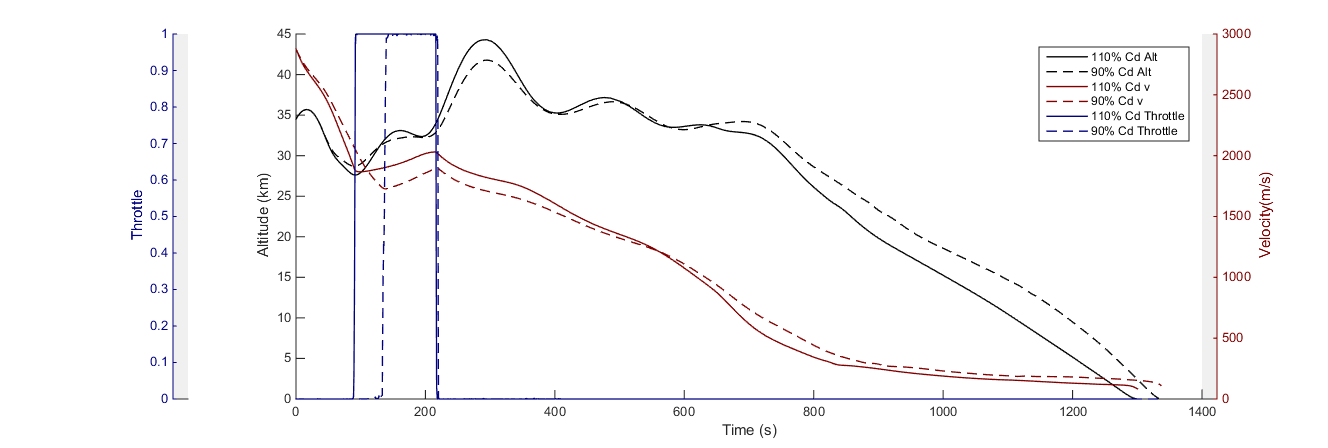
\includegraphics[width=0.9\linewidth]{Figures/CdVariation}
\caption{Comparison of optimal trajectories with $\pm10\%$ $C_D$ variance.}
\label{fig:CdVariation}
\end{figure}

\begin{figure}[ht]
\centering
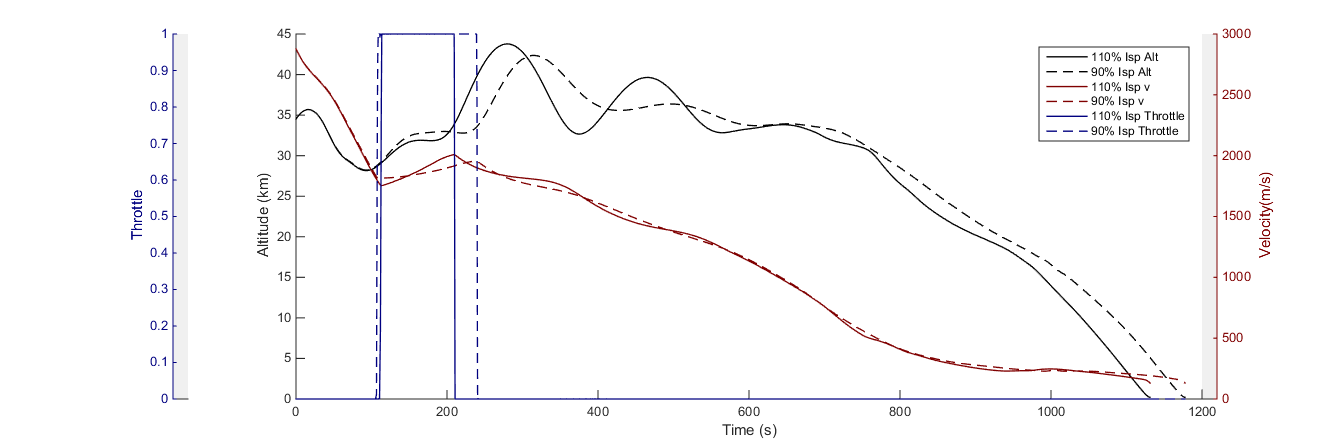
\includegraphics[width=0.9\linewidth]{Figures/IspVariation}
\caption{Comparison of optimal trajectories with $\pm10\%$ $I_{SP}$ variance.}
\label{fig:IspVariation}
\end{figure}



\section{Conclusion}
The fly-back trajectory of the SPARTAN hypersonic vehicle is investigated, from separation at 7.7$^\circ$S,145.0$^\circ$E to landing at 15.3$^\circ$S,144.9$^\circ$E, corresponding to a near 180$^\circ$ turn and a fly-back of 878km. The aerodynamics of the SPARTAN are calculated using CART3D, an inviscid CFD package, over the range of Mach numbers and angle of attack values of flight. The optimal trajectory of the SPARTAN is calculated, to fly-back to the initial launch position with minimum fuel. The optimal trajectory is calculated using the launch vehicle optimal control program LODESTAR. It is found that the SPARTAN is capable of returning to its initial launch position, using 166.0kg of fuel. The optimal trajectory terminates when SPARTAN reaches 200m altitude at a velocity of 119.8m/s. After this point, it is assumed that the SPARTAN lands on a traditional runway, at similar conditions to the space shuttle.  
This result indicates that the fly-back of a hypersonic launch vehicle from high velocity separation at a Mach number greater than nine, returning to its initial launch site using scramjet hypersonic airbreathing engines, is feasible. This fly-back to the the original launch site is a crucial component for low cost access-to-space using scramjets. 

The coefficient of drag of the SPARTAN and specific impulse of the scramjet engines were independently varied by $\pm10\%$ and the new optimal trajectories calculated to assess the robustness of the fly-back trajectory to uncertainties in vehicle aerodynamics and scramjet performance. It was found that a $\pm10\%$ variation in $C_D$ results in a +31.0\% or -34.9\% variation in fuel mass burned during fly-back, while a $\pm10\%$ variation in $I_{SP}$ results in a much smaller variation of -6.9\% or +13.8\%. These results indicate that the aerodynamics of a fly-back hypersonic accelerator are much more significant to the fly-back fuel usage than the performance of the scramjet engine. 

%\section*{Acknowledgments}
\section{Further Work}
This study assumes that the extra fuel necessary for the fly-back is able to be incorporated within the SPARTAN, and that the ascent is unchanged by the fly-back trajectory. However, realistically the additional fuel necessary for the fly-back will reduce the amount of fuel able to be used during the scramjet acceleration, and the ascent may be modified to mitigate the effects of the fly-back on total fuel consumption. A combined optimisation of the ascent and return trajectories is required to determine the impact of the return trajectory on the overall payload-to-orbit of the rocket-scramjet-rocket launch system. 

\bibliography{library}

\end{document}
